% Options for packages loaded elsewhere
\PassOptionsToPackage{unicode}{hyperref}
\PassOptionsToPackage{hyphens}{url}
\PassOptionsToPackage{dvipsnames,svgnames,x11names}{xcolor}
%
\documentclass[
  letterpaper,
  DIV=11,
  numbers=noendperiod]{scrreprt}

\usepackage{amsmath,amssymb}
\usepackage{iftex}
\ifPDFTeX
  \usepackage[T1]{fontenc}
  \usepackage[utf8]{inputenc}
  \usepackage{textcomp} % provide euro and other symbols
\else % if luatex or xetex
  \usepackage{unicode-math}
  \defaultfontfeatures{Scale=MatchLowercase}
  \defaultfontfeatures[\rmfamily]{Ligatures=TeX,Scale=1}
\fi
\usepackage{lmodern}
\ifPDFTeX\else  
    % xetex/luatex font selection
\fi
% Use upquote if available, for straight quotes in verbatim environments
\IfFileExists{upquote.sty}{\usepackage{upquote}}{}
\IfFileExists{microtype.sty}{% use microtype if available
  \usepackage[]{microtype}
  \UseMicrotypeSet[protrusion]{basicmath} % disable protrusion for tt fonts
}{}
\makeatletter
\@ifundefined{KOMAClassName}{% if non-KOMA class
  \IfFileExists{parskip.sty}{%
    \usepackage{parskip}
  }{% else
    \setlength{\parindent}{0pt}
    \setlength{\parskip}{6pt plus 2pt minus 1pt}}
}{% if KOMA class
  \KOMAoptions{parskip=half}}
\makeatother
\usepackage{xcolor}
\setlength{\emergencystretch}{3em} % prevent overfull lines
\setcounter{secnumdepth}{5}
% Make \paragraph and \subparagraph free-standing
\makeatletter
\ifx\paragraph\undefined\else
  \let\oldparagraph\paragraph
  \renewcommand{\paragraph}{
    \@ifstar
      \xxxParagraphStar
      \xxxParagraphNoStar
  }
  \newcommand{\xxxParagraphStar}[1]{\oldparagraph*{#1}\mbox{}}
  \newcommand{\xxxParagraphNoStar}[1]{\oldparagraph{#1}\mbox{}}
\fi
\ifx\subparagraph\undefined\else
  \let\oldsubparagraph\subparagraph
  \renewcommand{\subparagraph}{
    \@ifstar
      \xxxSubParagraphStar
      \xxxSubParagraphNoStar
  }
  \newcommand{\xxxSubParagraphStar}[1]{\oldsubparagraph*{#1}\mbox{}}
  \newcommand{\xxxSubParagraphNoStar}[1]{\oldsubparagraph{#1}\mbox{}}
\fi
\makeatother

\usepackage{color}
\usepackage{fancyvrb}
\newcommand{\VerbBar}{|}
\newcommand{\VERB}{\Verb[commandchars=\\\{\}]}
\DefineVerbatimEnvironment{Highlighting}{Verbatim}{commandchars=\\\{\}}
% Add ',fontsize=\small' for more characters per line
\usepackage{framed}
\definecolor{shadecolor}{RGB}{241,243,245}
\newenvironment{Shaded}{\begin{snugshade}}{\end{snugshade}}
\newcommand{\AlertTok}[1]{\textcolor[rgb]{0.68,0.00,0.00}{#1}}
\newcommand{\AnnotationTok}[1]{\textcolor[rgb]{0.37,0.37,0.37}{#1}}
\newcommand{\AttributeTok}[1]{\textcolor[rgb]{0.40,0.45,0.13}{#1}}
\newcommand{\BaseNTok}[1]{\textcolor[rgb]{0.68,0.00,0.00}{#1}}
\newcommand{\BuiltInTok}[1]{\textcolor[rgb]{0.00,0.23,0.31}{#1}}
\newcommand{\CharTok}[1]{\textcolor[rgb]{0.13,0.47,0.30}{#1}}
\newcommand{\CommentTok}[1]{\textcolor[rgb]{0.37,0.37,0.37}{#1}}
\newcommand{\CommentVarTok}[1]{\textcolor[rgb]{0.37,0.37,0.37}{\textit{#1}}}
\newcommand{\ConstantTok}[1]{\textcolor[rgb]{0.56,0.35,0.01}{#1}}
\newcommand{\ControlFlowTok}[1]{\textcolor[rgb]{0.00,0.23,0.31}{\textbf{#1}}}
\newcommand{\DataTypeTok}[1]{\textcolor[rgb]{0.68,0.00,0.00}{#1}}
\newcommand{\DecValTok}[1]{\textcolor[rgb]{0.68,0.00,0.00}{#1}}
\newcommand{\DocumentationTok}[1]{\textcolor[rgb]{0.37,0.37,0.37}{\textit{#1}}}
\newcommand{\ErrorTok}[1]{\textcolor[rgb]{0.68,0.00,0.00}{#1}}
\newcommand{\ExtensionTok}[1]{\textcolor[rgb]{0.00,0.23,0.31}{#1}}
\newcommand{\FloatTok}[1]{\textcolor[rgb]{0.68,0.00,0.00}{#1}}
\newcommand{\FunctionTok}[1]{\textcolor[rgb]{0.28,0.35,0.67}{#1}}
\newcommand{\ImportTok}[1]{\textcolor[rgb]{0.00,0.46,0.62}{#1}}
\newcommand{\InformationTok}[1]{\textcolor[rgb]{0.37,0.37,0.37}{#1}}
\newcommand{\KeywordTok}[1]{\textcolor[rgb]{0.00,0.23,0.31}{\textbf{#1}}}
\newcommand{\NormalTok}[1]{\textcolor[rgb]{0.00,0.23,0.31}{#1}}
\newcommand{\OperatorTok}[1]{\textcolor[rgb]{0.37,0.37,0.37}{#1}}
\newcommand{\OtherTok}[1]{\textcolor[rgb]{0.00,0.23,0.31}{#1}}
\newcommand{\PreprocessorTok}[1]{\textcolor[rgb]{0.68,0.00,0.00}{#1}}
\newcommand{\RegionMarkerTok}[1]{\textcolor[rgb]{0.00,0.23,0.31}{#1}}
\newcommand{\SpecialCharTok}[1]{\textcolor[rgb]{0.37,0.37,0.37}{#1}}
\newcommand{\SpecialStringTok}[1]{\textcolor[rgb]{0.13,0.47,0.30}{#1}}
\newcommand{\StringTok}[1]{\textcolor[rgb]{0.13,0.47,0.30}{#1}}
\newcommand{\VariableTok}[1]{\textcolor[rgb]{0.07,0.07,0.07}{#1}}
\newcommand{\VerbatimStringTok}[1]{\textcolor[rgb]{0.13,0.47,0.30}{#1}}
\newcommand{\WarningTok}[1]{\textcolor[rgb]{0.37,0.37,0.37}{\textit{#1}}}

\providecommand{\tightlist}{%
  \setlength{\itemsep}{0pt}\setlength{\parskip}{0pt}}\usepackage{longtable,booktabs,array}
\usepackage{calc} % for calculating minipage widths
% Correct order of tables after \paragraph or \subparagraph
\usepackage{etoolbox}
\makeatletter
\patchcmd\longtable{\par}{\if@noskipsec\mbox{}\fi\par}{}{}
\makeatother
% Allow footnotes in longtable head/foot
\IfFileExists{footnotehyper.sty}{\usepackage{footnotehyper}}{\usepackage{footnote}}
\makesavenoteenv{longtable}
\usepackage{graphicx}
\makeatletter
\newsavebox\pandoc@box
\newcommand*\pandocbounded[1]{% scales image to fit in text height/width
  \sbox\pandoc@box{#1}%
  \Gscale@div\@tempa{\textheight}{\dimexpr\ht\pandoc@box+\dp\pandoc@box\relax}%
  \Gscale@div\@tempb{\linewidth}{\wd\pandoc@box}%
  \ifdim\@tempb\p@<\@tempa\p@\let\@tempa\@tempb\fi% select the smaller of both
  \ifdim\@tempa\p@<\p@\scalebox{\@tempa}{\usebox\pandoc@box}%
  \else\usebox{\pandoc@box}%
  \fi%
}
% Set default figure placement to htbp
\def\fps@figure{htbp}
\makeatother
% definitions for citeproc citations
\NewDocumentCommand\citeproctext{}{}
\NewDocumentCommand\citeproc{mm}{%
  \begingroup\def\citeproctext{#2}\cite{#1}\endgroup}
\makeatletter
 % allow citations to break across lines
 \let\@cite@ofmt\@firstofone
 % avoid brackets around text for \cite:
 \def\@biblabel#1{}
 \def\@cite#1#2{{#1\if@tempswa , #2\fi}}
\makeatother
\newlength{\cslhangindent}
\setlength{\cslhangindent}{1.5em}
\newlength{\csllabelwidth}
\setlength{\csllabelwidth}{3em}
\newenvironment{CSLReferences}[2] % #1 hanging-indent, #2 entry-spacing
 {\begin{list}{}{%
  \setlength{\itemindent}{0pt}
  \setlength{\leftmargin}{0pt}
  \setlength{\parsep}{0pt}
  % turn on hanging indent if param 1 is 1
  \ifodd #1
   \setlength{\leftmargin}{\cslhangindent}
   \setlength{\itemindent}{-1\cslhangindent}
  \fi
  % set entry spacing
  \setlength{\itemsep}{#2\baselineskip}}}
 {\end{list}}
\usepackage{calc}
\newcommand{\CSLBlock}[1]{\hfill\break\parbox[t]{\linewidth}{\strut\ignorespaces#1\strut}}
\newcommand{\CSLLeftMargin}[1]{\parbox[t]{\csllabelwidth}{\strut#1\strut}}
\newcommand{\CSLRightInline}[1]{\parbox[t]{\linewidth - \csllabelwidth}{\strut#1\strut}}
\newcommand{\CSLIndent}[1]{\hspace{\cslhangindent}#1}

\KOMAoption{captions}{tableheading}
\makeatletter
\@ifpackageloaded{tcolorbox}{}{\usepackage[skins,breakable]{tcolorbox}}
\@ifpackageloaded{fontawesome5}{}{\usepackage{fontawesome5}}
\definecolor{quarto-callout-color}{HTML}{909090}
\definecolor{quarto-callout-note-color}{HTML}{0758E5}
\definecolor{quarto-callout-important-color}{HTML}{CC1914}
\definecolor{quarto-callout-warning-color}{HTML}{EB9113}
\definecolor{quarto-callout-tip-color}{HTML}{00A047}
\definecolor{quarto-callout-caution-color}{HTML}{FC5300}
\definecolor{quarto-callout-color-frame}{HTML}{acacac}
\definecolor{quarto-callout-note-color-frame}{HTML}{4582ec}
\definecolor{quarto-callout-important-color-frame}{HTML}{d9534f}
\definecolor{quarto-callout-warning-color-frame}{HTML}{f0ad4e}
\definecolor{quarto-callout-tip-color-frame}{HTML}{02b875}
\definecolor{quarto-callout-caution-color-frame}{HTML}{fd7e14}
\makeatother
\makeatletter
\@ifpackageloaded{bookmark}{}{\usepackage{bookmark}}
\makeatother
\makeatletter
\@ifpackageloaded{caption}{}{\usepackage{caption}}
\AtBeginDocument{%
\ifdefined\contentsname
  \renewcommand*\contentsname{Table of contents}
\else
  \newcommand\contentsname{Table of contents}
\fi
\ifdefined\listfigurename
  \renewcommand*\listfigurename{List of Figures}
\else
  \newcommand\listfigurename{List of Figures}
\fi
\ifdefined\listtablename
  \renewcommand*\listtablename{List of Tables}
\else
  \newcommand\listtablename{List of Tables}
\fi
\ifdefined\figurename
  \renewcommand*\figurename{Figure}
\else
  \newcommand\figurename{Figure}
\fi
\ifdefined\tablename
  \renewcommand*\tablename{Table}
\else
  \newcommand\tablename{Table}
\fi
}
\@ifpackageloaded{float}{}{\usepackage{float}}
\floatstyle{ruled}
\@ifundefined{c@chapter}{\newfloat{codelisting}{h}{lop}}{\newfloat{codelisting}{h}{lop}[chapter]}
\floatname{codelisting}{Listing}
\newcommand*\listoflistings{\listof{codelisting}{List of Listings}}
\makeatother
\makeatletter
\makeatother
\makeatletter
\@ifpackageloaded{caption}{}{\usepackage{caption}}
\@ifpackageloaded{subcaption}{}{\usepackage{subcaption}}
\makeatother
\makeatletter
\definecolor{QuartoInternalColor1}{rgb}{0.15,0.56,0.56}
\definecolor{QuartoInternalColor8}{rgb}{0.20,0.40,0.40}
\definecolor{QuartoInternalColor2}{rgb}{0,0,0}
\definecolor{QuartoInternalColor7}{rgb}{0.60,0.00,1.00}
\definecolor{QuartoInternalColor5}{rgb}{0.00,0.40,0.79}
\definecolor{QuartoInternalColor3}{rgb}{0.00,0.45,0.15}
\definecolor{QuartoInternalColor4}{rgb}{0.70,0.17,0.19}
\definecolor{QuartoInternalColor6}{rgb}{0.00,0.40,0.00}
\definecolor{QuartoInternalColor9}{rgb}{0.74,0.74,0.74}
\makeatother

\usepackage{bookmark}

\IfFileExists{xurl.sty}{\usepackage{xurl}}{} % add URL line breaks if available
\urlstyle{same} % disable monospaced font for URLs
\hypersetup{
  pdftitle={Introduction to Data Science},
  pdfauthor={Ethan Meyers},
  colorlinks=true,
  linkcolor={blue},
  filecolor={Maroon},
  citecolor={Blue},
  urlcolor={Blue},
  pdfcreator={LaTeX via pandoc}}


\title{Introduction to Data Science}
\author{Ethan Meyers}
\date{}

\begin{document}
\maketitle

\renewcommand*\contentsname{Table of contents}
{
\hypersetup{linkcolor=}
\setcounter{tocdepth}{2}
\tableofcontents
}

\bookmarksetup{startatroot}

\chapter*{Welcome}\label{welcome}
\addcontentsline{toc}{chapter}{Welcome}

\markboth{Welcome}{Welcome}


\includegraphics[width=3.125in,height=\textheight,keepaspectratio]{images/cover_img.png}

This book gives an introduction to Data Science using the Python
programming langauge.

\bookmarksetup{startatroot}

\chapter{Introduction}\label{introduction}

In this chapter we will discuss what the field of Data Science is, and
give a brief history of how the field developed.

This book is your guide to understanding the exciting and increasingly
influential field of data science. Whether you're curious about how data
shapes our world or are looking to explore the possibilities of
data-driven insights, this book will provide you with a foundational
understanding of what data science is and why it matters.

\section{What is Data Science?}\label{what-is-data-science}

Data science is a dynamic and interdisciplinary field that combines
techniques and theories from statistics, computer science, and
specialized knowledge in various areas to extract valuable knowledge and
insights from data {[}Chapter 1{]}. This data can come in many forms,
whether neatly organized in databases or existing as unstructured
information like text or images.

At its core, data science follows a systematic process for analyzing
data. This includes a range of crucial steps, starting with data
collection and ensuring the data is in a usable state through data
cleaning. Once prepared, the data is explored to uncover initial
patterns and relationships (data exploration). Data scientists then
apply various modeling techniques to identify deeper insights, which
need to be carefully interpreted to draw meaningful conclusions.
Finally, the findings are communicated effectively to inform decisions
and understanding {[}Chapter 1{]}.

The field of data science has experienced remarkable growth in recent
years This surge in prominence can be attributed to several key factors:
- The explosion in the amount of data being generated across all
sectors, from social media to scientific research. - Significant
advancements in computing power, enabling the processing and analysis of
these vast datasets. - The development of increasingly sophisticated
analytical tools and techniques that allow for more complex and
insightful data exploration.

By delving into data science, you can gain practical analytical skills
that are applicable across a wide array of fields {[}Chapter 1, 62{]}.
You'll learn how to approach real-world data, identify key questions,
and use data-driven methods to find answers and understand the world
around us {[}Chapter 1, 62{]}. As a lighthearted starting point, you
might hear the quip that ``A Data Scientist is a Statistician who lives
in San Francisco'' {[}Chapter 1, 11{]}. While humorous, this simple
definition hints at the combination of statistical thinking with the
technological innovation often associated with data science. Throughout
this book, we will move beyond simplistic definitions to explore the
rich and multifaceted nature of this vital field.

Key points - Despite the fact that humans have been collecting data for
millenia, and doing sophisticated analyses of data for centuries, the
field of data science'' (or at least the name) is relatively new. -

\section{A brief history of Data
Science}\label{a-brief-history-of-data-science}

\subsection{A brief history of data}\label{a-brief-history-of-data}

\subsection{A brief history of
Statistics}\label{a-brief-history-of-statistics}

\subsection{A brief history of
computation}\label{a-brief-history-of-computation}

Computational devices also have a long history.

\subsection{The creation of the field of Data
Science}\label{the-creation-of-the-field-of-data-science}

\bookmarksetup{startatroot}

\chapter{Literate programming and reproducible
research}\label{literate-programming-and-reproducible-research}

The concept of reproducible research has a rich history, rooted in the
broader scientific principle that results should be
verifiable/reproducible by others. As science became increasingly
computational in the late 20th century, the challenge of ensuring
reproducibility grew. Early computational research often involved custom
scripts, manual data manipulation, and undocumented workflows, making it
difficult for others to replicate results---even when code and data were
shared.

A foundational influence was Donald Knuth's idea of ``literate
programming'' in the 1980s. Knuth advocated for writing code and
documentation together, so that the logic and reasoning behind analyses
were transparent and accessible. This philosophy inspired later tools
that integrated narrative and computation.

In the 1990s and early 2000s, as computational analyses became more
central to fields like genomics, climate science, and economics, the
limitations of traditional publishing became apparent. Researchers like
Jon Claerbout and David Donoho were early advocates for reproducible
computational research, arguing that published results should include
the code and data necessary to regenerate all figures and analyses. This
led to the development of reproducible research standards and the first
``compendia''---bundled packages of code, data, and documentation.

The emergence of tools such as Sweave (for R and LaTeX), Jupyter
Notebooks (originally IPython), and RMarkdown in the 2000s and 2010s
marked a turning point. These platforms allowed researchers to combine
code, results, and explanatory text in a single, executable document.
This integration made it much easier to share analyses and ensure that
others could reproduce and build upon published work. More recently,
Quarto has extended these ideas, supporting multiple programming
languages and flexible publishing formats.

Despite advances in computational tools, the scientific community has
faced what is now known as the ``reproducibility crisis.'' Over the past
decade, numerous studies have revealed that a significant proportion of
published scientific findings cannot be independently reproduced or
replicated. This crisis has affected a wide range of disciplines, from
psychology and medicine to the natural and computational sciences.
Contributing factors include selective reporting, lack of transparency
in methods and data, insufficient documentation of code, and pressures
to publish novel results quickly.

The reproducibility crisis has highlighted the urgent need for more
transparent and verifiable research practices. As science became
increasingly computational in the late 20th century, ensuring
reproducibility grew more challenging. Early computational research
often involved custom scripts, manual data manipulation, and
undocumented workflows, making it difficult for others to replicate
results---even when code and data were shared.

The reproducibility crisis has prompted widespread calls for reform.
Funding agencies, journals, and professional societies now increasingly
require that data and code be made available, and that research
workflows be documented in detail. The adoption of version control
systems like Git, preregistration of studies, and open peer review are
among the practices being promoted to address these challenges.

Today, reproducible research is a cornerstone of open science. The
evolution of reproducible research reflects both technological advances
and a growing recognition of the importance of openness, transparency,
and trust in scientific discovery. By embracing reproducible practices,
the scientific community aims to restore confidence in published results
and accelerate the pace of reliable, cumulative knowledge.

\section{Jupyter notebooks}\label{jupyter-notebooks}

In this book we will be using Jupyter notebooks to do our data analyses.
These notebooks allow us to interleave ``code cells'' which contain
Python code, with ``Markdown cells'' which contain written explanations
for what our analyses are showing.

Jupyter notebooks are a powerful tool for interactive computing and
reproducible research. They provide an environment where you can write
and execute code, visualize data, and document your workflow all in one
place. This makes it easy to experiment with different analyses, see
immediate results, and keep a clear record of your work.

A typical Jupyter notebook consists of a sequence of cells. Code cells
let you write and run code in languages such as Python, R, or Julia.
When you run a code cell, the output---such as tables, plots, or
text---is displayed directly below the cell. Markdown cells, on the
other hand, are used for formatted text, explanations, equations (using
LaTeX), and images. This combination supports a narrative style of
analysis, where you can explain your reasoning alongside the code and
results.

Jupyter notebooks are widely used in data science, education, and
research because they encourage transparency and reproducibility. You
can share your notebooks with others, allowing them to rerun your
analyses, modify code, and build upon your work. Notebooks can be
exported to various formats, including HTML and PDF, making it easy to
present your findings.

Throughout this book, you will learn how to use Jupyter notebooks
effectively: running code, documenting your process, visualizing data,
and sharing your results. By mastering notebooks, you'll gain a valuable
skill for modern data science workflows.

\subsection{Using Jupyter notebooks}\label{using-jupyter-notebooks}

To use Jupyter notebooks, you interact with two main types of cells:
code cells and markdown cells.

\begin{itemize}
\item
  \textbf{Code cells}: These contain executable code (such as Python).
  To run a code cell, click on it and press \texttt{Shift+Enter} (or
  click the ``Run'' button in the toolbar). The output will appear
  directly below the cell. You can edit and rerun code cells as often as
  you like.
\item
  \textbf{Markdown cells}: These are used for formatted text,
  explanations, equations, and images. To edit a markdown cell,
  double-click it. After editing, press \texttt{Shift+Enter} to render
  the formatted text.
\end{itemize}

\textbf{Basic workflow:} 1. Add a new cell using the ``+'' button or
menu. 2. Choose the cell type (code or markdown) from the toolbar or
menu. 3. Write your code or text. 4. Run the cell with
\texttt{Shift+Enter}.

You can rearrange cells by dragging them, and you can delete or
duplicate cells using the cell menu. Notebooks automatically save your
work, but you can also save manually (\texttt{Ctrl+S}).

Jupyter notebooks support interactive features such as plotting,
widgets, and inline visualizations, making them ideal for data
exploration and analysis.

\bookmarksetup{startatroot}

\chapter{Python basics}\label{python-basics}

Now that we have discussed what data science is, let's learn some of the
basics of the Python programming language. Once we have learned some of
these Python basics we can begin to analyze data!

\section{Expressions}\label{expressions}

A \textbf{Python expression} is \textbf{any piece of code that produces
a value.}. For example, the following is an expression that simply
creates the number 21.

\begin{Shaded}
\begin{Highlighting}[]
\DecValTok{21}
\end{Highlighting}
\end{Shaded}

\begin{verbatim}
21
\end{verbatim}

Similarly, an expression could be a series of mathematical operations
that evaluate to number. For example, if want want to add 5 plus 2 and
then multiple the result by 6 we can write:

\begin{Shaded}
\begin{Highlighting}[]
\DecValTok{6} \OperatorTok{*}\NormalTok{ (}\DecValTok{5} \OperatorTok{+} \DecValTok{2}\NormalTok{) }
\end{Highlighting}
\end{Shaded}

\begin{verbatim}
42
\end{verbatim}

As mentioned above, the defining features of a \emph{python expression}
is that it produces a value. Expressions are one of the fundamental
building blocks of data analysis and they will appear frequently
throughout this book.

\begin{tcolorbox}[enhanced jigsaw, bottomtitle=1mm, colframe=quarto-callout-tip-color-frame, toptitle=1mm, colbacktitle=quarto-callout-tip-color!10!white, rightrule=.15mm, leftrule=.75mm, opacityback=0, breakable, coltitle=black, left=2mm, opacitybacktitle=0.6, titlerule=0mm, bottomrule=.15mm, title=\textcolor{quarto-callout-tip-color}{\faLightbulb}\hspace{0.5em}{Exercise}, arc=.35mm, colback=white, toprule=.15mm]

What would happen if we remove the parenthesis from the expression we
ran above and instead run \texttt{6\ *\ 5\ +\ 2}. See if you can predict
what the result will be and then try it out in Python by running the
code in a code cell and see if you get the result you predicted.

\end{tcolorbox}

\begin{tcolorbox}[enhanced jigsaw, bottomtitle=1mm, colframe=quarto-callout-note-color-frame, toptitle=1mm, colbacktitle=quarto-callout-note-color!10!white, rightrule=.15mm, leftrule=.75mm, opacityback=0, breakable, coltitle=black, left=2mm, opacitybacktitle=0.6, titlerule=0mm, bottomrule=.15mm, title=\textcolor{quarto-callout-note-color}{\faInfo}\hspace{0.5em}{Solution}, arc=.35mm, colback=white, toprule=.15mm]

\begin{Shaded}
\begin{Highlighting}[]
\DecValTok{6} \OperatorTok{*} \DecValTok{5} \OperatorTok{+} \DecValTok{2}
\end{Highlighting}
\end{Shaded}

\begin{verbatim}
32
\end{verbatim}

The result is 32, which makes sense because in the standard order of
mathematical operations, multiplication occurs before addition so we
multiple 6 * 5 and get 30, and then we add 2 to get 32.

\end{tcolorbox}

\subsection{Mathematical expressions}\label{mathematical-expressions}

The expressions shown above were all ``mathematical expressions''
because they involve calculating numeric quantities. We can also write
statements that will do operations on text and other types of data which
we will describe more below. But first, let's explore mathematical
expressions a bit more. Below is a table of some of the mathematical
operations that are part of

\begin{longtable}[]{@{}llll@{}}
\caption{Python mathematical
operators}\label{tbl-math-ops}\tabularnewline
\toprule\noalign{}
Operation & Symbol & Example & Result \\
\midrule\noalign{}
\endfirsthead
\toprule\noalign{}
Operation & Symbol & Example & Result \\
\midrule\noalign{}
\endhead
\bottomrule\noalign{}
\endlastfoot
Addition & + & 5 + 3 & 8 \\
Subtraction & - & 10 - 4 & 6 \\
Multiplication & * & 7 * 2 & 14 \\
Division & / & 12 / 5 & 2.4 \\
Exponentiation & ** & 3 ** 2 & 9 \\
Remainder & \% & 10 \% 3 & 1 \\
\end{longtable}

\begin{tcolorbox}[enhanced jigsaw, bottomtitle=1mm, colframe=quarto-callout-tip-color-frame, toptitle=1mm, colbacktitle=quarto-callout-tip-color!10!white, rightrule=.15mm, leftrule=.75mm, opacityback=0, breakable, coltitle=black, left=2mm, opacitybacktitle=0.6, titlerule=0mm, bottomrule=.15mm, title=\textcolor{quarto-callout-tip-color}{\faLightbulb}\hspace{0.5em}{Exercise}, arc=.35mm, colback=white, toprule=.15mm]

What is the remainder from dividing 365 by 7? Please write some Python
code that produces the answer.

\end{tcolorbox}

\begin{tcolorbox}[enhanced jigsaw, bottomtitle=1mm, colframe=quarto-callout-note-color-frame, toptitle=1mm, colbacktitle=quarto-callout-note-color!10!white, rightrule=.15mm, leftrule=.75mm, opacityback=0, breakable, coltitle=black, left=2mm, opacitybacktitle=0.6, titlerule=0mm, bottomrule=.15mm, title=\textcolor{quarto-callout-note-color}{\faInfo}\hspace{0.5em}{Solution}, arc=.35mm, colback=white, toprule=.15mm]

\begin{Shaded}
\begin{Highlighting}[]
\DecValTok{365} \OperatorTok{\%} \DecValTok{7}
\end{Highlighting}
\end{Shaded}

\begin{verbatim}
1
\end{verbatim}

\end{tcolorbox}

\section{Syntax}\label{syntax}

\textbf{Syntax} is the set of rules that defines how Python code
\textbf{must} be written. One that think of syntax as the grammar of the
Python programming language. In order for Python to be able to run your
code, it \textbf{must} use the correct syntax. If incorrect syntax is
used, then one will get a ``syntax error'', and the code will not run.

To illustrate this, let's calculate the value of 8 squared (\(8^2\))
which hopefully you remember is equal to the value of 64. As shown
Table~\ref{tbl-math-ops}, if we want to take a value \texttt{x} to the
power \texttt{y} (i.e., to calculate \(x^y\)) we use the syntax
\texttt{x**y}. So, if we wanted to calculate \(8^2\) we would write the
following Python code:

\begin{Shaded}
\begin{Highlighting}[]
\DecValTok{8}\OperatorTok{**}\DecValTok{2}
\end{Highlighting}
\end{Shaded}

\begin{verbatim}
64
\end{verbatim}

Since we have written the correct syntax, the code runs and the result
of 64 is calculated as expected.

However, if we accidentially put an extra space between the two
\texttt{*} symbols, Python will not know how to interpret the expression
and we will get a syntax error as shown below:

\begin{Shaded}
\begin{Highlighting}[]
\DecValTok{8}\OperatorTok{*} \OperatorTok{*}\DecValTok{2}
\end{Highlighting}
\end{Shaded}

\begin{Highlighting}
\textcolor{black}{SyntaxError: invalid syntax (3783800731.py, line 1)}
\textcolor{black}{  }\textcolor{QuartoInternalColor1}{Cell}\textcolor{QuartoInternalColor2}{}\textcolor{QuartoInternalColor1}{ }\textcolor{QuartoInternalColor2}{}\textcolor{QuartoInternalColor3}{In[6]}\textcolor{QuartoInternalColor2}{}\textcolor{QuartoInternalColor3}{, line 1}\textcolor{QuartoInternalColor2}{}
\textcolor{QuartoInternalColor2}{}\textcolor{QuartoInternalColor4}{    }\textcolor{QuartoInternalColor2}{}\textcolor{QuartoInternalColor4}{8* *2}\textcolor{QuartoInternalColor2}{}
\textcolor{QuartoInternalColor2}{       ^}
\textcolor{QuartoInternalColor2}{}\textcolor{QuartoInternalColor4}{SyntaxError}\textcolor{QuartoInternalColor2}{}\textcolor{QuartoInternalColor4}{:}\textcolor{QuartoInternalColor2}{ invalid syntax}
\end{Highlighting}

When there is a syntax error, Python will print out \texttt{SyntaxError}
and give you an indication where the syntax error has occurred using a
\^{} symbol.\footnote{The reason this is a syntax error is because
  Python inteprets a single \texttt{*} symbol as a multiplicaiton
  symbol. Thus it is trying to multiple 8 by another multiplication
  symbol \texttt{*}, which gives an error since one can only multiply
  two numbers together.} As we can see here, Python is trying to show
that the syntax error has occurred due to the extra space between the *
symbols.

The ability to be able to spot and fix syntax errors is a fundamental
skill you will develop as become proficient in analyzing data in Python.

\section{Assignment statements}\label{assignment-statements}

An \emph{assignment statement} is a line of code that is used to store a
value in a named \textbf{variable}. We can then refer back to this
variable name to retrieve the value we have stored.

To assign a value to a variable we use the \texttt{=} symbol. For
example, the following code assigns the value \texttt{10} to the
variable \texttt{a}:

\begin{Shaded}
\begin{Highlighting}[]
\NormalTok{a }\OperatorTok{=} \DecValTok{10}
\end{Highlighting}
\end{Shaded}

We can then refer back to the variable \texttt{a} later in our code to
retrive the stored value. For example, if we just write \texttt{a} by
itself on the last line of our Python code cell, it will print out the
value stored in \texttt{a}.

\begin{Shaded}
\begin{Highlighting}[]
\NormalTok{a}
\end{Highlighting}
\end{Shaded}

\begin{verbatim}
10
\end{verbatim}

As we can see, the value printed out is \texttt{10} which is the value
we had previously stored in the name \texttt{a}.

If we were to assign the name \texttt{a} to another value, it will
overwrite the previously stored value and \texttt{a} will store the new
value.

\begin{Shaded}
\begin{Highlighting}[]
\NormalTok{a }\OperatorTok{=} \DecValTok{21}
\NormalTok{a}
\end{Highlighting}
\end{Shaded}

\begin{verbatim}
21
\end{verbatim}

We an also do mathematical operations on values stored in variables,
such as adding and multiplying variables together. For example, we can
assign the variable \texttt{h} to store the value 24, and the variable
\texttt{d} to store the value 7, and then we can multiple these together
and store the result in the variable \texttt{t}.

\begin{Shaded}
\begin{Highlighting}[]
\NormalTok{h }\OperatorTok{=} \DecValTok{24}
\NormalTok{d }\OperatorTok{=} \DecValTok{7}
\NormalTok{t }\OperatorTok{=}\NormalTok{ h }\OperatorTok{*}\NormalTok{ d}
\NormalTok{t}
\end{Highlighting}
\end{Shaded}

\begin{verbatim}
168
\end{verbatim}

\begin{tcolorbox}[enhanced jigsaw, bottomtitle=1mm, colframe=quarto-callout-tip-color-frame, toptitle=1mm, colbacktitle=quarto-callout-tip-color!10!white, rightrule=.15mm, leftrule=.75mm, opacityback=0, breakable, coltitle=black, left=2mm, opacitybacktitle=0.6, titlerule=0mm, bottomrule=.15mm, title=\textcolor{quarto-callout-tip-color}{\faLightbulb}\hspace{0.5em}{Exercise}, arc=.35mm, colback=white, toprule=.15mm]

In the above code we calculated \texttt{t\ =\ h\ *\ d}. Which of the
following do you think will happen to the value stored in \texttt{t} if
we change the value of h to 3? I.e., if we run the following code, what
do you think it will print out?

\begin{Shaded}
\begin{Highlighting}[]
\NormalTok{h }\OperatorTok{=} \DecValTok{3}
\NormalTok{t}
\end{Highlighting}
\end{Shaded}

\begin{enumerate}
\def\labelenumi{\alph{enumi}.}
\tightlist
\item
  The value of \texttt{t} will be change to be 21 (i.e.,
  \texttt{7\ *\ 3}).
\item
  The value of \texttt{t} will not change and will still contain
  \texttt{168}.
\item
  Something else will happen (e.g., Python will give an error).
\end{enumerate}

\end{tcolorbox}

\begin{tcolorbox}[enhanced jigsaw, bottomtitle=1mm, colframe=quarto-callout-note-color-frame, toptitle=1mm, colbacktitle=quarto-callout-note-color!10!white, rightrule=.15mm, leftrule=.75mm, opacityback=0, breakable, coltitle=black, left=2mm, opacitybacktitle=0.6, titlerule=0mm, bottomrule=.15mm, title=\textcolor{quarto-callout-note-color}{\faInfo}\hspace{0.5em}{Solution}, arc=.35mm, colback=white, toprule=.15mm]

\begin{Shaded}
\begin{Highlighting}[]
\NormalTok{h }\OperatorTok{=} \DecValTok{3}
\NormalTok{t}
\end{Highlighting}
\end{Shaded}

\begin{verbatim}
168
\end{verbatim}

As you can see, the value of \texttt{t} did not change. This illustrates
an important point that once a value is calculated and stored in a
variable it will not change if the variable that were used as part of
the calculation are updated!

\end{tcolorbox}

\subsection{Variable names}\label{variable-names}

Variable names in Python must follow certain rules:

\begin{itemize}
\tightlist
\item
  Must start with a letter (a-z, A-Z) or an underscore (\_), but not a
  number.
\item
  Can contain letters, numbers, and underscores.
\item
  Cannot contain spaces or special characters (like \texttt{@},
  \texttt{\#}, \texttt{\$}, etc.).
\item
  Cannot be a reserved Python keyword that are part of the Python
  language (like \texttt{for}, \texttt{if}, \texttt{class}, etc.).
\end{itemize}

If these rules are not followed, Python will produce a syntax error

It's also important to use meaningful variable names. For example,
\texttt{t} is technically a valid variable name but it is not
descriptive, while \texttt{total\_hours} is much clearer. Using
meaningful names makes your code easier to read and understand.

\begin{tcolorbox}[enhanced jigsaw, bottomtitle=1mm, colframe=quarto-callout-tip-color-frame, toptitle=1mm, colbacktitle=quarto-callout-tip-color!10!white, rightrule=.15mm, leftrule=.75mm, opacityback=0, breakable, coltitle=black, left=2mm, opacitybacktitle=0.6, titlerule=0mm, bottomrule=.15mm, title=\textcolor{quarto-callout-tip-color}{\faLightbulb}\hspace{0.5em}{Exercise}, arc=.35mm, colback=white, toprule=.15mm]

The minimum wage in the United States in 2025 is \$7.25. If someone
works 40 hours per week for all 52 weeks in a year, what would there
yearly earnings be? Please calculate by creating \emph{meaningful}
variable names for:

\begin{enumerate}
\def\labelenumi{\arabic{enumi}.}
\tightlist
\item
  The minimum wage amount\\
\item
  The number of hours in a week\\
\item
  The number of weeks in a year
\end{enumerate}

Then calculate the total yearly wage and store this result in another
meaningful variable name, and print out the value stored in this last
variable. Hint: Using underscores \texttt{\_} in your variable names is
highly encouraged to make them more readible.

\end{tcolorbox}

\begin{tcolorbox}[enhanced jigsaw, bottomtitle=1mm, colframe=quarto-callout-note-color-frame, toptitle=1mm, colbacktitle=quarto-callout-note-color!10!white, rightrule=.15mm, leftrule=.75mm, opacityback=0, breakable, coltitle=black, left=2mm, opacitybacktitle=0.6, titlerule=0mm, bottomrule=.15mm, title=\textcolor{quarto-callout-note-color}{\faInfo}\hspace{0.5em}{Solution}, arc=.35mm, colback=white, toprule=.15mm]

\begin{Shaded}
\begin{Highlighting}[]
\NormalTok{hours }\OperatorTok{=} \DecValTok{24}
\NormalTok{days }\OperatorTok{=} \DecValTok{7}
\NormalTok{total\_hours\_in\_a\_week }\OperatorTok{=}\NormalTok{ hours }\OperatorTok{*}\NormalTok{ days}
\NormalTok{total\_hours\_in\_a\_week}
\end{Highlighting}
\end{Shaded}

\begin{verbatim}
168
\end{verbatim}

\end{tcolorbox}

\section{Comments}\label{comments}

Another very useful feature in Python is the ability to add
\textbf{comments} to your code. Comments are lines in your code that are
ignored by Python when your code runs. They are used to explain what
your code is doing, make notes to yourself, or leave instructions for
others who may read your code in the future.

In Python, you create a comment by starting the line with the
\texttt{\#} symbol. Anything after the \texttt{\#} on that line will be
treated as a comment and not executed.

For example:

\begin{Shaded}
\begin{Highlighting}[]
\CommentTok{\# The code below calculates the number of seconds in a day}
\NormalTok{seconds\_in\_a\_day }\OperatorTok{=} \DecValTok{60} \OperatorTok{*} \DecValTok{60} \OperatorTok{*} \DecValTok{24}

\NormalTok{seconds\_in\_a\_day}
\end{Highlighting}
\end{Shaded}

\begin{verbatim}
86400
\end{verbatim}

We will use comments extensively throughout this book to explain what
code is doing and to make our code easier to understand. Adding clear
comments is a good habit that will help both you and others who read
your code in the future, so we strongly encourage you to add comments
liberally for all code you write.

\section{Functions (call expressions)}\label{functions-call-expressions}

A \textbf{function} is a reusable piece of code that performs a specific
task. You can think of a function as a ``machine'' that takes some
input, does something with it, and then gives you an output.

Python comes with many built-in functions that you can use right away,
and you can also load in additional functions in packages that other
people have written. You can also write own functions, which is a topic
we will discuss later in this book.

To use a function, you ``call'' it by writing its name followed by
parentheses. If the function needs information to do its job, you put
that information (called ``arguments'') inside the parentheses.

For example, the \texttt{abs()} function take in a number and returns
the absolute value of the number.

\begin{Shaded}
\begin{Highlighting}[]
\BuiltInTok{abs}\NormalTok{(}\OperatorTok{{-}}\DecValTok{10}\NormalTok{)}
\end{Highlighting}
\end{Shaded}

\begin{verbatim}
10
\end{verbatim}

Some functions can take in multiple arguments. When multiple arguments
are provided, they are separated by commas within the parentheses. For
example, the \texttt{min()} function can take several numbers and will
return the smallest one:

\begin{Shaded}
\begin{Highlighting}[]
\BuiltInTok{min}\NormalTok{(}\DecValTok{10}\NormalTok{, }\DecValTok{2}\NormalTok{, }\DecValTok{87}\NormalTok{, }\DecValTok{5}\NormalTok{, }\DecValTok{90}\NormalTok{)}
\end{Highlighting}
\end{Shaded}

\begin{verbatim}
2
\end{verbatim}

Another useful function is the \texttt{print()} function for displaying
multiple pieces of information in a single Jupyter notebook code cell.
By default, Jupyter will only display the result of the last line in a
code cell. If you want to display multiple values or add custom
messages, you can use the \texttt{print()} function.

For example, the code below will print both the numbers \texttt{2} and
\texttt{3} in the same code cell. If we did not use the \texttt{print()}
function, only the number \texttt{3} would be printed since it is the
last line in the cell, but the number 2 would not be printed because it
is on the last line in the cell.

\begin{Shaded}
\begin{Highlighting}[]
\CommentTok{\# We need to call print() explicitly here to print the value of }
\CommentTok{\# 2 since it is not on the last line of the code cell}

\BuiltInTok{print}\NormalTok{(}\DecValTok{2}\NormalTok{)  }



\CommentTok{\# The value of 3 will be printed here without needing to call }
\CommentTok{\# the print() function because it is the last line in the cell}

\DecValTok{3}
\end{Highlighting}
\end{Shaded}

\begin{verbatim}
2
\end{verbatim}

\begin{verbatim}
3
\end{verbatim}

\begin{tcolorbox}[enhanced jigsaw, bottomtitle=1mm, colframe=quarto-callout-tip-color-frame, toptitle=1mm, colbacktitle=quarto-callout-tip-color!10!white, rightrule=.15mm, leftrule=.75mm, opacityback=0, breakable, coltitle=black, left=2mm, opacitybacktitle=0.6, titlerule=0mm, bottomrule=.15mm, title=\textcolor{quarto-callout-tip-color}{\faLightbulb}\hspace{0.5em}{Exercise}, arc=.35mm, colback=white, toprule=.15mm]

Try using the \texttt{print()} function to display both a message and a
value in the same output. For example, print the message ``The answer
is:'' followed by the result of \texttt{6\ *\ 7}.

\end{tcolorbox}

\begin{tcolorbox}[enhanced jigsaw, bottomtitle=1mm, colframe=quarto-callout-note-color-frame, toptitle=1mm, colbacktitle=quarto-callout-note-color!10!white, rightrule=.15mm, leftrule=.75mm, opacityback=0, breakable, coltitle=black, left=2mm, opacitybacktitle=0.6, titlerule=0mm, bottomrule=.15mm, title=\textcolor{quarto-callout-note-color}{\faInfo}\hspace{0.5em}{Solution}, arc=.35mm, colback=white, toprule=.15mm]

\begin{Shaded}
\begin{Highlighting}[]
\BuiltInTok{print}\NormalTok{(}\StringTok{"The answer is:"}\NormalTok{)}
\DecValTok{6} \OperatorTok{*} \DecValTok{7}
\end{Highlighting}
\end{Shaded}

\begin{verbatim}
The answer is:
\end{verbatim}

\begin{verbatim}
42
\end{verbatim}

\begin{Shaded}
\begin{Highlighting}[]
\CommentTok{\# We can also print multiple pieces of text on a single line by }
\CommentTok{\# passing multiple arguments to the print() function: }

\BuiltInTok{print}\NormalTok{(}\StringTok{"The answer is:"}\NormalTok{, }\DecValTok{6} \OperatorTok{*} \DecValTok{7}\NormalTok{)}
\end{Highlighting}
\end{Shaded}

\begin{verbatim}
The answer is: 42
\end{verbatim}

\end{tcolorbox}

\section{Data types}\label{data-types}

Python is able to process many different types of data, referred to as
``data types''. So, far we have only explored numeric data. Let's
continue exploring numerical data in a little more detial and then we
will go on to examine other types of data.

\subsection{Numbers}\label{numbers}

Python uses two different formats to store numerical data known as
``integers'' and ``floating-point numbers''.

\begin{itemize}
\tightlist
\item
  \textbf{Integers} (\texttt{int}): Whole numbers without a decimal
  point, such as \texttt{5}, \texttt{-3}, or \texttt{1000}.
\item
  \textbf{Floating-point numbers} (\texttt{float}): Numbers that have a
  decimal point, such as \texttt{3.14}, \texttt{-0.5}, or \texttt{2.0}.
\end{itemize}

We can tell if a number is a floating point number (i.e., a ``float'')
by seeing if there is a decimal point at the end of the number when we
print out the number.

\begin{Shaded}
\begin{Highlighting}[]
\CommentTok{\# This is an integer, which we can tell becaues there is no decimal point}
\DecValTok{5}
\end{Highlighting}
\end{Shaded}

\begin{verbatim}
5
\end{verbatim}

\begin{Shaded}
\begin{Highlighting}[]
\CommentTok{\# Although we are dividing two integers, the result is a floating point number}
\CommentTok{\# which we can tell becaues there is a decimal point}

\DecValTok{10}\OperatorTok{/}\DecValTok{2}
\end{Highlighting}
\end{Shaded}

\begin{verbatim}
5.0
\end{verbatim}

We can also use the \texttt{type()} function to check if a number is an
integer or a floating point number.

\begin{Shaded}
\begin{Highlighting}[]
\CommentTok{\# This is a floating point number}

\BuiltInTok{type}\NormalTok{(}\FloatTok{5.0}\NormalTok{)}
\end{Highlighting}
\end{Shaded}

\begin{verbatim}
float
\end{verbatim}

When analyzing the data, usually it does not matter if Python is storing
a number as an integer or a floating point number since Python does the
math sensibly and converts between integers and floating point numbers
as needed. However, internally Python is representing these number is
quite different ways.

More imporantly is to know that there are some limitations to the way
Python stores both integers and floats. In particular, both of these
types of numbers are represented using a finite amount of memory, so
there is a largest number integer that can be represented and a limit to
the precision of floating-point numbers. For most practical purposes,
these limits are very large, but you may encounter issues with extremely
large numbers or with floating-point arithmetic where results are not
exactly as expected due to rounding errors.

For example, if we multiple intergers that are too long, we can get a
\texttt{ValueError} which indicates that Python is running into problems
representing an integer this large.

\begin{Shaded}
\begin{Highlighting}[]
\CommentTok{\# There is a limited size to integers (although the size is pretty large)}

\DecValTok{1234567} \OperatorTok{**} \DecValTok{890} 
\end{Highlighting}
\end{Shaded}

\begin{Highlighting}
\textcolor{black}{ValueError: Exceeds the limit (4300 digits) for integer string conversion; use sys.set_int_max_str_digits() to increase the limit}
\textcolor{black}{}\textcolor{QuartoInternalColor4}{---------------------------------------------------------------------------}\textcolor{QuartoInternalColor2}{}
\textcolor{QuartoInternalColor2}{}\textcolor{QuartoInternalColor4}{ValueError}\textcolor{QuartoInternalColor2}{                                Traceback (most recent call last)}
\textcolor{QuartoInternalColor2}{}\textcolor{QuartoInternalColor1}{File }\textcolor{QuartoInternalColor2}{}\textcolor{QuartoInternalColor3}{c:\Users\em939\Desktop\git_repos\books_to_write\intro_datasci_vscode\.venv\Lib\site-packages\IPython\core\formatters.py:770}\textcolor{QuartoInternalColor2}{, in }\textcolor{QuartoInternalColor1}{PlainTextFormatter.__call__}\textcolor{QuartoInternalColor2}{}\textcolor{QuartoInternalColor5}{(self, obj)}\textcolor{QuartoInternalColor2}{}
\textcolor{QuartoInternalColor2}{}\textcolor{QuartoInternalColor3}{    763}\textcolor{QuartoInternalColor2}{ stream = StringIO()}
\textcolor{QuartoInternalColor2}{}\textcolor{QuartoInternalColor3}{    764}\textcolor{QuartoInternalColor2}{ printer = pretty.RepresentationPrinter(stream, }\textcolor{QuartoInternalColor6}{self}\textcolor{QuartoInternalColor2}{.verbose,}
\textcolor{QuartoInternalColor2}{}\textcolor{QuartoInternalColor3}{    765}\textcolor{QuartoInternalColor2}{     }\textcolor{QuartoInternalColor6}{self}\textcolor{QuartoInternalColor2}{.max_width, }\textcolor{QuartoInternalColor6}{self}\textcolor{QuartoInternalColor2}{.newline,}
\textcolor{QuartoInternalColor2}{}\textcolor{QuartoInternalColor3}{    766}\textcolor{QuartoInternalColor2}{     max_seq_length=}\textcolor{QuartoInternalColor6}{self}\textcolor{QuartoInternalColor2}{.max_seq_length,}
\textcolor{QuartoInternalColor2}{}\textcolor{QuartoInternalColor3}{    767}\textcolor{QuartoInternalColor2}{     singleton_pprinters=}\textcolor{QuartoInternalColor6}{self}\textcolor{QuartoInternalColor2}{.singleton_printers,}
\textcolor{QuartoInternalColor2}{}\textcolor{QuartoInternalColor3}{    768}\textcolor{QuartoInternalColor2}{     type_pprinters=}\textcolor{QuartoInternalColor6}{self}\textcolor{QuartoInternalColor2}{.type_printers,}
\textcolor{QuartoInternalColor2}{}\textcolor{QuartoInternalColor3}{    769}\textcolor{QuartoInternalColor2}{     deferred_pprinters=}\textcolor{QuartoInternalColor6}{self}\textcolor{QuartoInternalColor2}{.deferred_printers)}
\textcolor{QuartoInternalColor2}{}\textcolor{QuartoInternalColor3}{--> }\textcolor{QuartoInternalColor2}{}\textcolor{QuartoInternalColor3}{770}\textcolor{QuartoInternalColor2}{ }\textcolor{QuartoInternalColor2}{printer}\textcolor{QuartoInternalColor2}{}\textcolor{QuartoInternalColor2}{.}\textcolor{QuartoInternalColor2}{}\textcolor{QuartoInternalColor2}{pretty}\textcolor{QuartoInternalColor2}{}\textcolor{QuartoInternalColor2}{(}\textcolor{QuartoInternalColor2}{}\textcolor{QuartoInternalColor2}{obj}\textcolor{QuartoInternalColor2}{}\textcolor{QuartoInternalColor2}{)}\textcolor{QuartoInternalColor2}{}
\textcolor{QuartoInternalColor2}{}\textcolor{QuartoInternalColor3}{    771}\textcolor{QuartoInternalColor2}{ printer.flush()}
\textcolor{QuartoInternalColor2}{}\textcolor{QuartoInternalColor3}{    772}\textcolor{QuartoInternalColor2}{ }\textcolor{QuartoInternalColor6}{return}\textcolor{QuartoInternalColor2}{ stream.getvalue()}
\textcolor{QuartoInternalColor2}{}\textcolor{QuartoInternalColor1}{File }\textcolor{QuartoInternalColor2}{}\textcolor{QuartoInternalColor3}{c:\Users\em939\Desktop\git_repos\books_to_write\intro_datasci_vscode\.venv\Lib\site-packages\IPython\lib\pretty.py:386}\textcolor{QuartoInternalColor2}{, in }\textcolor{QuartoInternalColor1}{RepresentationPrinter.pretty}\textcolor{QuartoInternalColor2}{}\textcolor{QuartoInternalColor5}{(self, obj)}\textcolor{QuartoInternalColor2}{}
\textcolor{QuartoInternalColor2}{}\textcolor{QuartoInternalColor3}{    383}\textcolor{QuartoInternalColor2}{ }\textcolor{QuartoInternalColor6}{for}\textcolor{QuartoInternalColor2}{ }\textcolor{QuartoInternalColor6}{cls}\textcolor{QuartoInternalColor2}{ }\textcolor{QuartoInternalColor7}{in}\textcolor{QuartoInternalColor2}{ _get_mro(obj_class):}
\textcolor{QuartoInternalColor2}{}\textcolor{QuartoInternalColor3}{    384}\textcolor{QuartoInternalColor2}{     }\textcolor{QuartoInternalColor6}{if}\textcolor{QuartoInternalColor2}{ }\textcolor{QuartoInternalColor6}{cls}\textcolor{QuartoInternalColor2}{ }\textcolor{QuartoInternalColor7}{in}\textcolor{QuartoInternalColor2}{ }\textcolor{QuartoInternalColor6}{self}\textcolor{QuartoInternalColor2}{.type_pprinters:}
\textcolor{QuartoInternalColor2}{}\textcolor{QuartoInternalColor3}{    385}\textcolor{QuartoInternalColor2}{         }\textcolor{QuartoInternalColor8}{# printer registered in self.type_pprinters}\textcolor{QuartoInternalColor2}{}
\textcolor{QuartoInternalColor2}{}\textcolor{QuartoInternalColor3}{--> }\textcolor{QuartoInternalColor2}{}\textcolor{QuartoInternalColor3}{386}\textcolor{QuartoInternalColor2}{         }\textcolor{QuartoInternalColor6}{return}\textcolor{QuartoInternalColor2}{ }\textcolor{QuartoInternalColor6}{self}\textcolor{QuartoInternalColor2}{}\textcolor{QuartoInternalColor2}{.}\textcolor{QuartoInternalColor2}{}\textcolor{QuartoInternalColor2}{type_pprinters}\textcolor{QuartoInternalColor2}{}\textcolor{QuartoInternalColor2}{[}\textcolor{QuartoInternalColor2}{}\textcolor{QuartoInternalColor6}{cls}\textcolor{QuartoInternalColor2}{}\textcolor{QuartoInternalColor2}{]}\textcolor{QuartoInternalColor2}{}\textcolor{QuartoInternalColor2}{(}\textcolor{QuartoInternalColor2}{}\textcolor{QuartoInternalColor2}{obj}\textcolor{QuartoInternalColor2}{}\textcolor{QuartoInternalColor2}{,}\textcolor{QuartoInternalColor2}{}\textcolor{QuartoInternalColor2}{ }\textcolor{QuartoInternalColor2}{}\textcolor{QuartoInternalColor6}{self}\textcolor{QuartoInternalColor2}{}\textcolor{QuartoInternalColor2}{,}\textcolor{QuartoInternalColor2}{}\textcolor{QuartoInternalColor2}{ }\textcolor{QuartoInternalColor2}{}\textcolor{QuartoInternalColor2}{cycle}\textcolor{QuartoInternalColor2}{}\textcolor{QuartoInternalColor2}{)}\textcolor{QuartoInternalColor2}{}
\textcolor{QuartoInternalColor2}{}\textcolor{QuartoInternalColor3}{    387}\textcolor{QuartoInternalColor2}{     }\textcolor{QuartoInternalColor6}{else}\textcolor{QuartoInternalColor2}{:}
\textcolor{QuartoInternalColor2}{}\textcolor{QuartoInternalColor3}{    388}\textcolor{QuartoInternalColor2}{         }\textcolor{QuartoInternalColor8}{# deferred printer}\textcolor{QuartoInternalColor2}{}
\textcolor{QuartoInternalColor2}{}\textcolor{QuartoInternalColor3}{    389}\textcolor{QuartoInternalColor2}{         printer = }\textcolor{QuartoInternalColor6}{self}\textcolor{QuartoInternalColor2}{._in_deferred_types(}\textcolor{QuartoInternalColor6}{cls}\textcolor{QuartoInternalColor2}{)}
\textcolor{QuartoInternalColor2}{}\textcolor{QuartoInternalColor1}{File }\textcolor{QuartoInternalColor2}{}\textcolor{QuartoInternalColor3}{c:\Users\em939\Desktop\git_repos\books_to_write\intro_datasci_vscode\.venv\Lib\site-packages\IPython\lib\pretty.py:786}\textcolor{QuartoInternalColor2}{, in }\textcolor{QuartoInternalColor1}{_repr_pprint}\textcolor{QuartoInternalColor2}{}\textcolor{QuartoInternalColor5}{(obj, p, cycle)}\textcolor{QuartoInternalColor2}{}
\textcolor{QuartoInternalColor2}{}\textcolor{QuartoInternalColor3}{    784}\textcolor{QuartoInternalColor2}{ }\textcolor{QuartoInternalColor9}{}\textcolor{QuartoInternalColor2}{}\textcolor{QuartoInternalColor2}{"""A pprint that just redirects to the normal repr function."""}\textcolor{QuartoInternalColor2}{}
\textcolor{QuartoInternalColor2}{}\textcolor{QuartoInternalColor3}{    785}\textcolor{QuartoInternalColor2}{ }\textcolor{QuartoInternalColor8}{# Find newlines and replace them with p.break_()}\textcolor{QuartoInternalColor2}{}
\textcolor{QuartoInternalColor2}{}\textcolor{QuartoInternalColor3}{--> }\textcolor{QuartoInternalColor2}{}\textcolor{QuartoInternalColor3}{786}\textcolor{QuartoInternalColor2}{ output = }\textcolor{QuartoInternalColor6}{repr}\textcolor{QuartoInternalColor2}{}\textcolor{QuartoInternalColor2}{(}\textcolor{QuartoInternalColor2}{}\textcolor{QuartoInternalColor2}{obj}\textcolor{QuartoInternalColor2}{}\textcolor{QuartoInternalColor2}{)}\textcolor{QuartoInternalColor2}{}
\textcolor{QuartoInternalColor2}{}\textcolor{QuartoInternalColor3}{    787}\textcolor{QuartoInternalColor2}{ lines = output.splitlines()}
\textcolor{QuartoInternalColor2}{}\textcolor{QuartoInternalColor3}{    788}\textcolor{QuartoInternalColor2}{ }\textcolor{QuartoInternalColor6}{with}\textcolor{QuartoInternalColor2}{ p.group():}
\textcolor{QuartoInternalColor2}{}\textcolor{QuartoInternalColor4}{ValueError}\textcolor{QuartoInternalColor2}{: Exceeds the limit (4300 digits) for integer string conversion; use sys.set_int_max_str_digits() to increase the limit}
\end{Highlighting}

Simiarly, if we try to create a floating-point number with too many
decimal points the number will be truncated, although no error is given,
so one needs to be careful if very high precision is needed in a
calculation.

\begin{Shaded}
\begin{Highlighting}[]
\CommentTok{\# There is a limited precision to floating point numbers (the last digits are trucated)}

\FloatTok{.12345678901234567890123456789} 
\end{Highlighting}
\end{Shaded}

\begin{verbatim}
0.12345678901234568
\end{verbatim}

We can also convert numbers between integers and floating point numbers
using the \texttt{int()} and \texttt{float()} functions. When converting
from a floating point number to an integer using teh \texttt{int()}
function, one needs to be aware that the decimal part of the number will
be removed (i.e., rounded down to the closest integer)

\begin{Shaded}
\begin{Highlighting}[]
\CommentTok{\# Convert an integer to a floating point number.  We can see the conversion worked because the number is printed with a decimal point. }

\BuiltInTok{float}\NormalTok{(}\DecValTok{5}\NormalTok{)}
\end{Highlighting}
\end{Shaded}

\begin{verbatim}
5.0
\end{verbatim}

\begin{Shaded}
\begin{Highlighting}[]
\CommentTok{\# Convert a floating point number to an integer. Note that the decimal part of the number is removed}

\BuiltInTok{int}\NormalTok{(}\FloatTok{3.14159}\NormalTok{)}
\end{Highlighting}
\end{Shaded}

\begin{verbatim}
3
\end{verbatim}

Finally, one should be aware that Python sometimes prints out numbers
using scientific notation. Scientific notation is a way of writing very
large or very small numbers more compactly, using the letter \texttt{e}
to indicate ``times ten to the power of.'' For example, \texttt{2.5e6}
means (2.5 \times 10\^{}\{6\}), or \texttt{2,500,000}. Similarly,
\texttt{3e-09} means (3 \times 10\^{}\{-9\}), or \texttt{0.000000003}.
Python will automatically use this notation when displaying numbers that
are extremely large or small.

\begin{Shaded}
\begin{Highlighting}[]
\CommentTok{\# The output is in scientific notation}
\DecValTok{30} \OperatorTok{/} \DecValTok{4000000000} 
\end{Highlighting}
\end{Shaded}

\begin{verbatim}
7.5e-09
\end{verbatim}

\begin{tcolorbox}[enhanced jigsaw, bottomtitle=1mm, colframe=quarto-callout-tip-color-frame, toptitle=1mm, colbacktitle=quarto-callout-tip-color!10!white, rightrule=.15mm, leftrule=.75mm, opacityback=0, breakable, coltitle=black, left=2mm, opacitybacktitle=0.6, titlerule=0mm, bottomrule=.15mm, title=\textcolor{quarto-callout-tip-color}{\faLightbulb}\hspace{0.5em}{Exercise}, arc=.35mm, colback=white, toprule=.15mm]

Take the square root of 12 and then square the result; i.e., calculate
\((\sqrt{12})^2\). Does Python return the correct result?

Hint: Note that you can calculate the square root of a number by taking
a number to the 1/2 power; i.e., \(\sqrt{12} = 12^{0.5}\)

\end{tcolorbox}

\begin{tcolorbox}[enhanced jigsaw, bottomtitle=1mm, colframe=quarto-callout-note-color-frame, toptitle=1mm, colbacktitle=quarto-callout-note-color!10!white, rightrule=.15mm, leftrule=.75mm, opacityback=0, breakable, coltitle=black, left=2mm, opacitybacktitle=0.6, titlerule=0mm, bottomrule=.15mm, title=\textcolor{quarto-callout-note-color}{\faInfo}\hspace{0.5em}{Solution}, arc=.35mm, colback=white, toprule=.15mm]

\begin{Shaded}
\begin{Highlighting}[]
\NormalTok{(}\DecValTok{12}\OperatorTok{**}\FloatTok{.5}\NormalTok{)}\OperatorTok{**}\DecValTok{2}
\end{Highlighting}
\end{Shaded}

\begin{verbatim}
11.999999999999998
\end{verbatim}

As you can see, there is slight imprecision here so we get a result of
11.999999999999998 rather than a value of 12.

\end{tcolorbox}

\subsection{Character strings}\label{character-strings}

A \textbf{character string} (or simply ``string'') is a sequence of
characters that are used to represent text, such as words, sentences, or
any other sequence of characters. Strings in Pythong are enclosed in
either single quotes (\texttt{\textquotesingle{}...\textquotesingle{}})
or double quotes (\texttt{"..."}). However, your string must start and
end with the same quote type; i.e., if the string starts with a single
quote tit also ends with a single quote, and the same for double quotes.

The following are valid strings in Python:

\begin{Shaded}
\begin{Highlighting}[]
\CommentTok{\textquotesingle{}This is a valid Python string with single quotes\textquotesingle{}}

\CommentTok{"This is another valid Python string using double quotes."}
\end{Highlighting}
\end{Shaded}

\begin{verbatim}
'This is another valid Python string using double quotes.'
\end{verbatim}

While using single or double quotes gives the same result, there are
cases where it is natural to use one over the other. For example, if
your string contains an apostrophe (single quote), it's easier to use
double quotes:

\begin{Shaded}
\begin{Highlighting}[]
\CommentTok{"This string contains an apostrophe: it\textquotesingle{}s easy to read."}
\end{Highlighting}
\end{Shaded}

\begin{verbatim}
"This string contains an apostrophe: it's easy to read."
\end{verbatim}

And if your string contains double quotes, it is easier to single quotes
when creating your string:

\begin{Shaded}
\begin{Highlighting}[]
\CommentTok{\textquotesingle{}She said, "Hello, world!"\textquotesingle{}}
\end{Highlighting}
\end{Shaded}

\begin{verbatim}
'She said, "Hello, world!"'
\end{verbatim}

We can also perform operations on strings, such as concatenation
(joining strings together). For example, to join two strings together,
you can use the \texttt{+} operator:

\begin{Shaded}
\begin{Highlighting}[]
\CommentTok{"water"} \OperatorTok{+} \StringTok{"mellon"}
\end{Highlighting}
\end{Shaded}

\begin{verbatim}
'watermellon'
\end{verbatim}

Note that the \texttt{+} operator we have used to concatenate strings is
the same \texttt{+} operator we used to add numbers. This illustrates an
important principle that an operator can behave differently depending on
the type of data it is used with. In Python, this is called ``operator
overloading.'' For numbers, \texttt{+} performs addition, while for
strings, it performs concatenation (joining the strings together).

\begin{tcolorbox}[enhanced jigsaw, bottomtitle=1mm, colframe=quarto-callout-tip-color-frame, toptitle=1mm, colbacktitle=quarto-callout-tip-color!10!white, rightrule=.15mm, leftrule=.75mm, opacityback=0, breakable, coltitle=black, left=2mm, opacitybacktitle=0.6, titlerule=0mm, bottomrule=.15mm, title=\textcolor{quarto-callout-tip-color}{\faLightbulb}\hspace{0.5em}{Exercise}, arc=.35mm, colback=white, toprule=.15mm]

Above we have seen that the \texttt{+} operator can behave differently
depending on whether it is operating on numbers or strings. We have also
seen that \texttt{*} operator is used to multiple two numbers together.
Do you think that the \texttt{*} operator will also work on strings?
Please write down, or say outloud whether you think the \texttt{*}
operator will work on strings, then see if your prediction is correct by
running the following code:

\begin{Shaded}
\begin{Highlighting}[]
\CommentTok{\textquotesingle{}ha\textquotesingle{}} \OperatorTok{*} \DecValTok{5}
\end{Highlighting}
\end{Shaded}

\begin{verbatim}
'hahahahaha'
\end{verbatim}

\end{tcolorbox}

\begin{tcolorbox}[enhanced jigsaw, bottomtitle=1mm, colframe=quarto-callout-note-color-frame, toptitle=1mm, colbacktitle=quarto-callout-note-color!10!white, rightrule=.15mm, leftrule=.75mm, opacityback=0, breakable, coltitle=black, left=2mm, opacitybacktitle=0.6, titlerule=0mm, bottomrule=.15mm, title=\textcolor{quarto-callout-note-color}{\faInfo}\hspace{0.5em}{Solution}, arc=.35mm, colback=white, toprule=.15mm]

\begin{Shaded}
\begin{Highlighting}[]
\CommentTok{\textquotesingle{}ha\textquotesingle{}} \OperatorTok{*} \DecValTok{5}
\end{Highlighting}
\end{Shaded}

\begin{verbatim}
'hahahahaha'
\end{verbatim}

As you can see, the \texttt{*} operator works on strings by repeating
the string the specified number of times. In this case,
\texttt{\textquotesingle{}ha\textquotesingle{}\ *\ 5} produces
\texttt{\textquotesingle{}hahahahaha\textquotesingle{}} (which is very
amusing).

\end{tcolorbox}

\subsubsection{String conversions}\label{string-conversions}

We can also convert strings into numbers and numbers into strings.

\subsubsection{String functions and
methods}\label{string-functions-and-methods}

\subsection{Booleans}\label{booleans}

You can check the type of a value in Python using the \texttt{type()}
function:

\section{Lists}\label{lists}

\subsection{Sequences}\label{sequences}

A sequence in Pythong is\ldots{}

A list is also a squence

\section{Other data structures}\label{other-data-structures}

\subsection{Tuples}\label{tuples}

\subsection{Dictionaries}\label{dictionaries}

\bookmarksetup{startatroot}

\chapter{Descriptive statistics and
plots}\label{descriptive-statistics-and-plots}

Now that we have covered some of the basic Python syntax we are ready to
start analyzing some data.

\bookmarksetup{startatroot}

\chapter{Array computations}\label{array-computations}

This is a book created from markdown and executable code.

\begin{Shaded}
\begin{Highlighting}[]
\ImportTok{import}\NormalTok{ matplotlib.pyplot }\ImportTok{as}\NormalTok{ plt}
\ImportTok{import}\NormalTok{ numpy }\ImportTok{as}\NormalTok{ np}
\NormalTok{eruptions }\OperatorTok{=}\NormalTok{ [}\DecValTok{1492}\NormalTok{, }\DecValTok{1585}\NormalTok{, }\DecValTok{1646}\NormalTok{, }\DecValTok{1677}\NormalTok{, }\DecValTok{1712}\NormalTok{, }\DecValTok{1949}\NormalTok{, }\DecValTok{1971}\NormalTok{, }\DecValTok{2021}\NormalTok{]}
\end{Highlighting}
\end{Shaded}

\begin{Shaded}
\begin{Highlighting}[]
\NormalTok{plt.figure(figsize}\OperatorTok{=}\NormalTok{(}\DecValTok{6}\NormalTok{, }\DecValTok{1}\NormalTok{))}
\NormalTok{plt.eventplot(eruptions, lineoffsets}\OperatorTok{=}\DecValTok{0}\NormalTok{, linelengths}\OperatorTok{=}\FloatTok{0.1}\NormalTok{, color}\OperatorTok{=}\StringTok{\textquotesingle{}black\textquotesingle{}}\NormalTok{)}
\NormalTok{plt.gca().axes.get\_yaxis().set\_visible(}\VariableTok{False}\NormalTok{)}
\NormalTok{plt.ylabel(}\StringTok{\textquotesingle{}\textquotesingle{}}\NormalTok{)}
\NormalTok{plt.show()}
\end{Highlighting}
\end{Shaded}

\begin{figure}[H]

\centering{

\pandocbounded{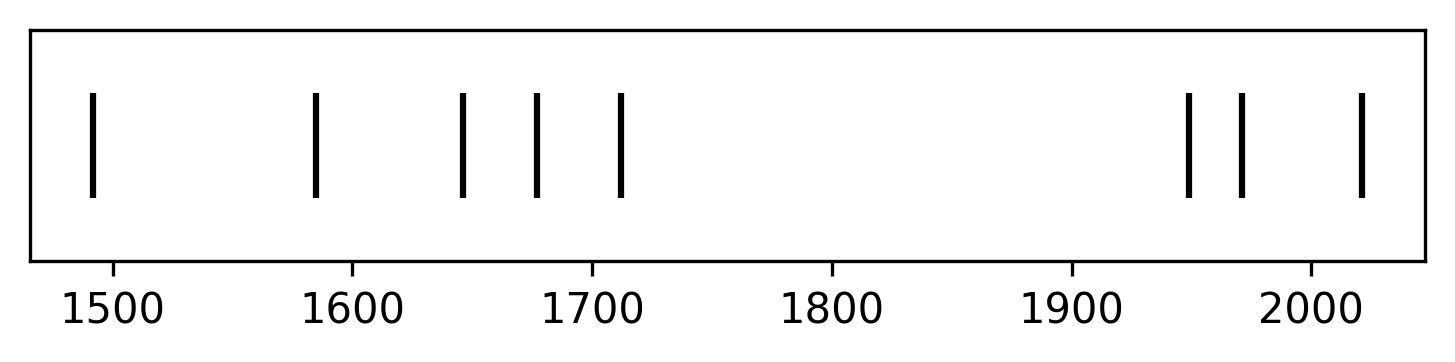
\includegraphics[keepaspectratio]{array_computations_files/figure-pdf/fig-timeline-output-1.png}}

}

\caption{\label{fig-timeline}Timeline of recent earthquakes on La Palma}

\end{figure}%

\begin{Shaded}
\begin{Highlighting}[]
\NormalTok{avg\_years\_between\_eruptions }\OperatorTok{=}\NormalTok{ np.mean(np.diff(eruptions[:}\OperatorTok{{-}}\DecValTok{1}\NormalTok{]))}
\NormalTok{avg\_years\_between\_eruptions}
\end{Highlighting}
\end{Shaded}

Based on data up to and including 1971, eruptions on La Palma happen
every 79.8 years on average.

Studies of the magma systems feeding the volcano, such as Marrero et al.
(2019), have proposed that there are two main magma reservoirs feeding
the Cumbre Vieja volcano; one in the mantle (30-40km depth) which
charges and in turn feeds a shallower crustal reservoir (10-20km depth).

Eight eruptions have been recorded since the late 1400s
(Figure~\ref{fig-timeline}).

Data and methods are discussed in Section~\ref{sec-data-methods}.

Let \(x\) denote the number of eruptions in a year. Then, \(x\) can be
modeled by a Poisson distribution

where \(\lambda\) is the rate of eruptions per year.

\begin{longtable}[]{@{}ll@{}}
\caption{Recent historic eruptions on La
Palma}\label{tbl-history}\tabularnewline
\toprule\noalign{}
Name & Year \\
\midrule\noalign{}
\endfirsthead
\toprule\noalign{}
Name & Year \\
\midrule\noalign{}
\endhead
\bottomrule\noalign{}
\endlastfoot
Current & 2021 \\
Teneguía & 1971 \\
Nambroque & 1949 \\
El Charco & 1712 \\
Volcán San Antonio & 1677 \\
Volcán San Martin & 1646 \\
Tajuya near El Paso & 1585 \\
Montaña Quemada & 1492 \\
\end{longtable}

Table~\ref{tbl-history} summarises the eruptions recorded since the
colonization of the islands by Europeans in the late 1400s.

\begin{figure}

\centering{

\pandocbounded{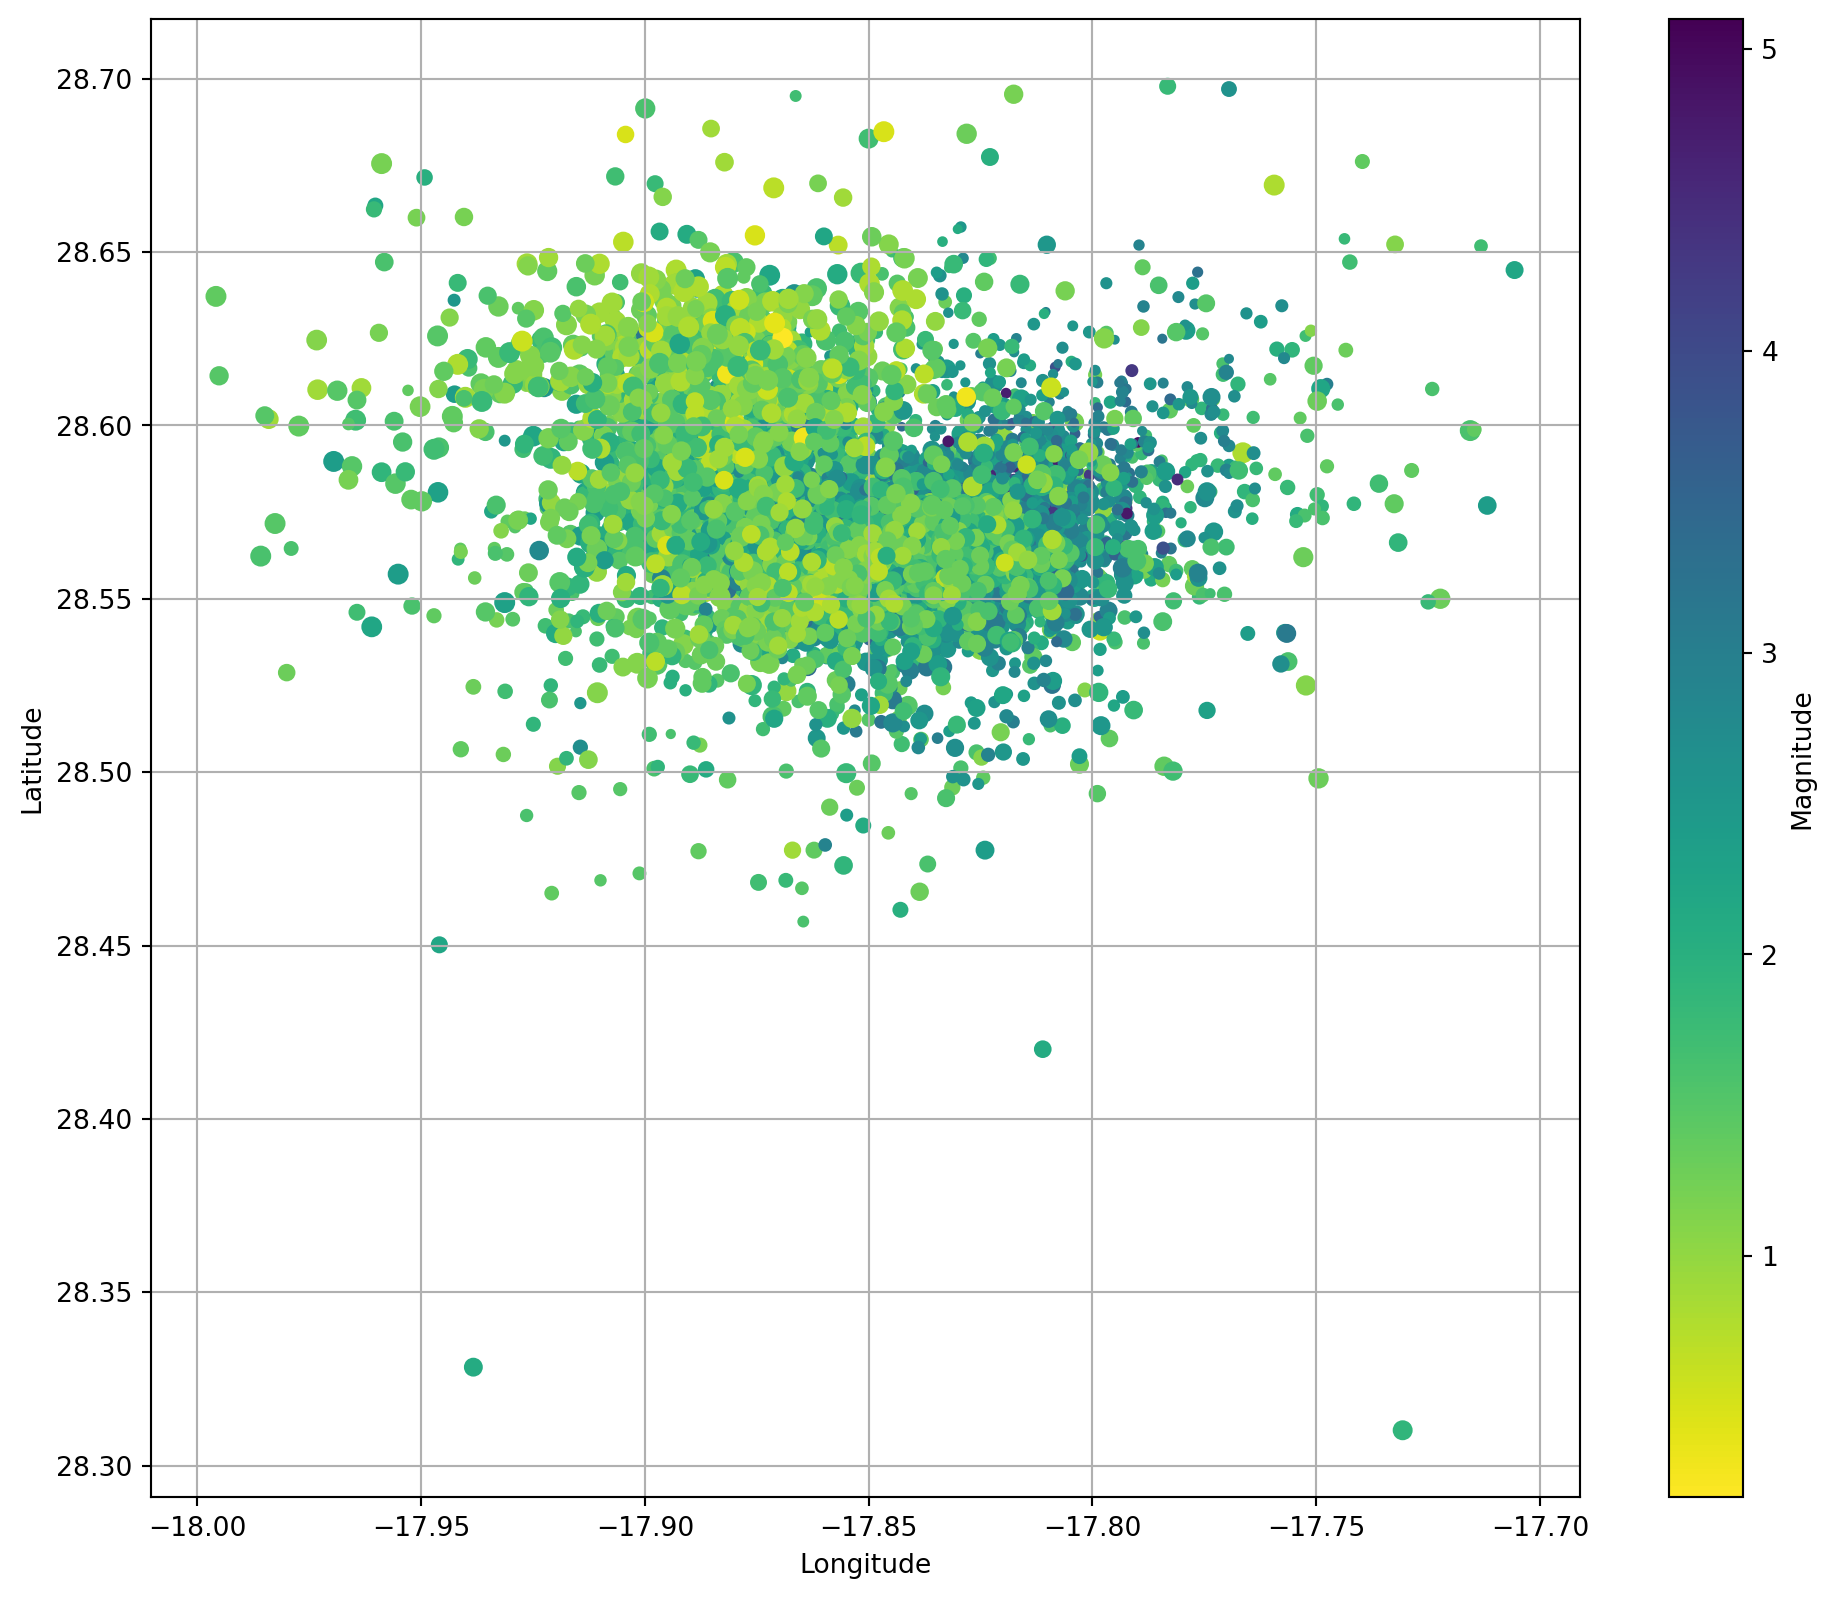
\includegraphics[keepaspectratio]{array_computations_files/figure-latex/notebooks-data-screening-fig-spatial-plot-output-1.png}}

}

\caption{\label{fig-spatial-plot}Locations of earthquakes on La Palma
since 2017.}

\end{figure}%

Figure~\ref{fig-spatial-plot} shows the location of recent Earthquakes
on La Palma.

\section{Data \& Methods}\label{sec-data-methods}

\section{Conclusion}\label{conclusion}

\section*{References}\label{references}
\addcontentsline{toc}{section}{References}

\markright{References}

\phantomsection\label{refs}
\begin{CSLReferences}{1}{0}
\bibitem[\citeproctext]{ref-marrero2019}
Marrero, José, Alicia García, Manuel Berrocoso, Ángeles Llinares,
Antonio Rodríguez-Losada, and R. Ortiz. 2019. {``Strategies for the
Development of Volcanic Hazard Maps in Monogenetic Volcanic Fields: The
Example of {La} {Palma} ({Canary} {Islands}).''} \emph{Journal of
Applied Volcanology} 8 (July).
\url{https://doi.org/10.1186/s13617-019-0085-5}.

\end{CSLReferences}

\bookmarksetup{startatroot}

\chapter{Data tables}\label{data-tables}

\bookmarksetup{startatroot}

\chapter{Data visualization}\label{data-visualization}




\end{document}
